
\begin{figure}
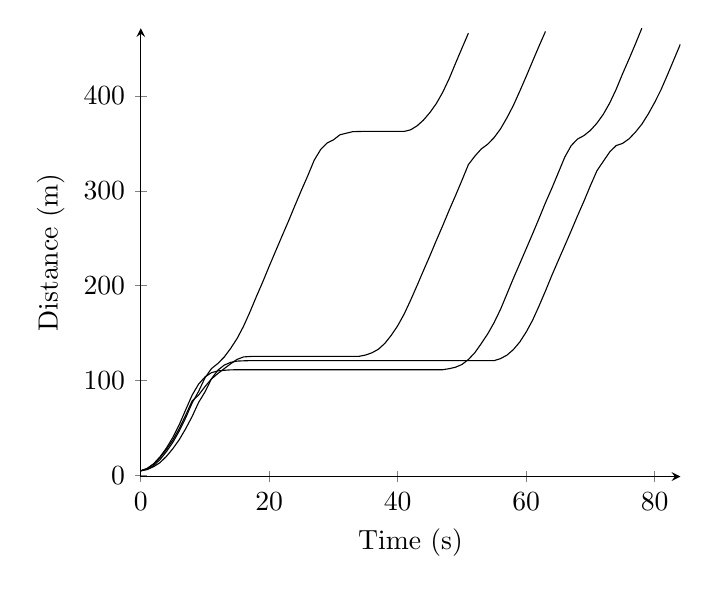
\begin{tikzpicture}
\begin{axis}[
legend style={anchor=west},
axis x line=bottom,
axis y line=left,
ymin=-1,
xlabel=Time (s),
ylabel=Distance (m),
]
\addplot[] coordinates {
(0, 5.1)
(1, 7.5271988438)
(2, 12.4290552295)
(3, 19.8013586611)
(4, 29.0869829261)
(5, 40.3898460728)
(6, 53.7896676259)
(7, 69.4608978891)
(8, 84.8354484508)
(9, 96.3727089924)
(10, 103.903210475)
(11, 108.394059789)
(12, 110.341371561)
(13, 110.943001569)
(14, 111.414896339)
(15, 111.521614828)
(16, 111.552952927)
(17, 111.566474559)
(18, 111.566474559)
(19, 111.566474559)
(20, 111.566474559)
(21, 111.566474559)
(22, 111.566474559)
(23, 111.566474559)
(24, 111.566474559)
(25, 111.566474559)
(26, 111.566474559)
(27, 111.566474559)
(28, 111.566474559)
(29, 111.566474559)
(30, 111.566474559)
(31, 111.566474559)
(32, 111.566474559)
(33, 111.566474559)
(34, 111.566474559)
(35, 111.566474559)
(36, 111.566474559)
(37, 111.566474559)
(38, 111.566474559)
(39, 111.566474559)
(40, 111.566474559)
(41, 111.566474559)
(42, 111.566474559)
(43, 111.566474559)
(44, 111.566474559)
(45, 111.566474559)
(46, 111.566474559)
(47, 111.566474559)
(48, 112.62408424)
(49, 114.181990424)
(50, 117.068698358)
(51, 122.312079388)
(52, 129.442930787)
(53, 139.060766653)
(54, 149.181039657)
(55, 161.174379285)
(56, 175.130713826)
(57, 191.387750841)
(58, 207.731525973)
(59, 223.329761807)
(60, 239.015528063)
(61, 254.795926808)
(62, 270.919856327)
(63, 287.486041974)
(64, 302.848596316)
(65, 319.125614692)
(66, 335.474190022)
(67, 347.584560319)
(68, 354.616159419)
(69, 358.196947752)
(70, 363.721352272)
(71, 371.168103204)
(72, 380.620969103)
(73, 392.498651046)
(74, 406.820064032)
(75, 423.266133755)
(76, 438.739035476)
(77, 454.707104931)
(78, 471.276471016)
};
\addplot[] coordinates {
(0, 5.1)
(1, 7.47378668564)
(2, 12.3011033111)
(3, 19.1380851255)
(4, 27.5864432411)
(5, 37.4820405503)
(6, 49.7048762399)
(7, 63.8079209619)
(8, 78.6907617097)
(9, 84.7955128547)
(10, 93.775023513)
(11, 101.778922819)
(12, 107.529070524)
(13, 112.729225547)
(14, 117.856115151)
(15, 122.450717575)
(16, 125.009143421)
(17, 125.505687522)
(18, 125.640155606)
(19, 125.663759839)
(20, 125.679423157)
(21, 125.679423157)
(22, 125.679423157)
(23, 125.679423157)
(24, 125.679423157)
(25, 125.679423157)
(26, 125.679423157)
(27, 125.679423157)
(28, 125.679423157)
(29, 125.679423157)
(30, 125.679423157)
(31, 125.679423157)
(32, 125.679423157)
(33, 125.679423157)
(34, 125.679423157)
(35, 127.02316054)
(36, 129.411728124)
(37, 133.149837786)
(38, 139.331637171)
(39, 147.870792743)
(40, 157.918637028)
(41, 170.156614987)
(42, 184.696946707)
(43, 200.071573029)
(44, 215.900955054)
(45, 231.410192725)
(46, 247.571954522)
(47, 263.228405228)
(48, 279.51478274)
(49, 295.061758487)
(50, 311.093897825)
(51, 327.628885681)
(52, 336.462249902)
(53, 344.060157562)
(54, 349.101138742)
(55, 356.038320061)
(56, 365.250209744)
(57, 376.93405035)
(58, 389.95182056)
(59, 404.980771372)
(60, 420.524390247)
(61, 436.603161127)
(62, 452.517505584)
(63, 467.928835049)
};
\addplot[] coordinates {
(0, 5.1)
(1, 6.64794521688)
(2, 10.604013155)
(3, 16.8715697212)
(4, 25.3387005178)
(5, 35.09948407)
(6, 47.1002858978)
(7, 60.9414103286)
(8, 76.5624079599)
(9, 88.6706239734)
(10, 103.081708874)
(11, 112.684545516)
(12, 118.123866617)
(13, 124.992146293)
(14, 134.059139644)
(15, 144.468318432)
(16, 157.325043025)
(17, 172.458353933)
(18, 188.643075168)
(19, 204.212261271)
(20, 220.667750252)
(21, 236.589004521)
(22, 252.489206759)
(23, 268.170710304)
(24, 284.518694824)
(25, 300.505342179)
(26, 315.925648021)
(27, 332.298527096)
(28, 343.439478302)
(29, 350.383273688)
(30, 353.724503971)
(31, 359.016082858)
(32, 360.695300202)
(33, 362.304465454)
(34, 362.532324247)
(35, 362.565564693)
(36, 362.579806629)
(37, 362.579806629)
(38, 362.579806629)
(39, 362.579806629)
(40, 362.579806629)
(41, 362.579806629)
(42, 364.235143067)
(43, 368.375490572)
(44, 374.46080127)
(45, 382.344076537)
(46, 391.854322321)
(47, 403.758992725)
(48, 418.008411912)
(49, 434.327243999)
(50, 450.305565665)
(51, 465.994445616)
};
\addplot[] coordinates {
(0, 5.1)
(1, 6.40291894428)
(2, 9.40776895606)
(3, 13.685732902)
(4, 20.3070943656)
(5, 28.4253595562)
(6, 37.9534234239)
(7, 49.5142514316)
(8, 62.328737855)
(9, 77.0002945628)
(10, 88.2199340577)
(11, 101.918391963)
(12, 111.035826318)
(13, 116.439303303)
(14, 119.336839376)
(15, 120.625029967)
(16, 120.934193957)
(17, 121.11409813)
(18, 121.11409813)
(19, 121.11409813)
(20, 121.11409813)
(21, 121.11409813)
(22, 121.11409813)
(23, 121.11409813)
(24, 121.11409813)
(25, 121.11409813)
(26, 121.11409813)
(27, 121.11409813)
(28, 121.11409813)
(29, 121.11409813)
(30, 121.11409813)
(31, 121.11409813)
(32, 121.11409813)
(33, 121.11409813)
(34, 121.11409813)
(35, 121.11409813)
(36, 121.11409813)
(37, 121.11409813)
(38, 121.11409813)
(39, 121.11409813)
(40, 121.11409813)
(41, 121.11409813)
(42, 121.11409813)
(43, 121.11409813)
(44, 121.11409813)
(45, 121.11409813)
(46, 121.11409813)
(47, 121.11409813)
(48, 121.11409813)
(49, 121.11409813)
(50, 121.11409813)
(51, 121.11409813)
(52, 121.11409813)
(53, 121.11409813)
(54, 121.11409813)
(55, 121.11409813)
(56, 123.221481788)
(57, 126.902879936)
(58, 132.718112007)
(59, 140.778044049)
(60, 151.268359249)
(61, 163.757399665)
(62, 178.745648252)
(63, 194.533463719)
(64, 211.063049909)
(65, 226.706035725)
(66, 242.194394118)
(67, 257.854431021)
(68, 273.854062166)
(69, 289.276946493)
(70, 305.553476926)
(71, 320.976083507)
(72, 331.085507345)
(73, 340.924740667)
(74, 347.652345366)
(75, 349.960297721)
(76, 354.72594746)
(77, 361.769756012)
(78, 370.202711207)
(79, 380.929310667)
(80, 393.162822391)
(81, 406.717155793)
(82, 422.290777421)
(83, 438.440430568)
(84, 454.512886592)
};

\end{axis}
\end{tikzpicture}
\label{tik:distance:0:13}
\caption{0 percent diving with GSC on route $13$}
\end{figure}
